\section{MQ NMR dynamics of spins-1/2 in a nanopore at low temperatures}
\label{sec:mq_dyn}

The standard MQ NMR experiment consists of four distinct periods of time (Fig.~\ref{fig:experiment}): preparation ($\tau$), evolution ($t_1$), mixing ($\tau$) and detection ($t_2$) \cite{mq_nmr_experiment}.
\begin{figure}
    \centering
    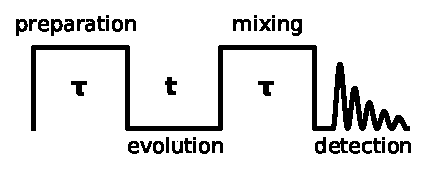
\includegraphics[width=\linewidth]{pic/experiment.pdf}
    \caption{The basic scheme of the MQ NMR experiment.}
    \label{fig:experiment}
\end{figure}
MQ coherences are created by a multi-pulse sequence irradiating the system on the preparation period \cite{mq_nmr_experiment}. Since the correlation time of the molecular diffusion of spin-carrying atoms (molecules) in nanopores is much shorter than both the dipolar time $t \approx \omega^{-1}_{\mathrm{loc}}$ ( $\omega^{-1}_{\mathrm{loc}}$  is the dipolar local field in the frequency units \cite{Goldman}) and  the period of the multi-pulse sequence on the preparation period of the MQ NMR experiment \cite{mq_nmr_experiment}, one can assume that spin dynamics is governed by the averaged dipolar coupling constant, $D$, which is the same for all spin pairs. Then the averaged non-secular two-spin/two-quantum Hamiltonian, $H_\mathrm{MQ}$, describing MQ dynamics on the preparation period, can be written in the rotating reference frame \cite{Goldman} as \cite{lab:mq_nmr_dyn_in_nanopores_2009}

\begin{equation}
    \label{eq:ham_mq}
    H_\mathrm{MQ}  = - \frac D 4 \left\{(I^+)^2 + (I^-)^2\right\},
\end{equation}
where  $I^{\pm} = \sum\limits_{j=1}^N I^{\pm}_j$, $N$ is the number of the spins in the nanopore, and $I^{\pm}_j$ are the raising/lowering operators of spin j.

In order to investigate the MQ NMR dynamics of the system one should find the density matrix $\rho(\tau)$ on the preparation period of the MQ NMR experiment \cite{mq_nmr_experiment} by solving the Liouville evolution equation \cite{lab:mq_mnr_qinfo_2012}

\begin{equation}
    \label{eq:liouvile}
    i \dfrac{d\rho(\tau)}{d \tau} = 
    \left[H_\mathrm{MQ}, \rho(\tau)\right]
\end{equation}
with the initial thermodynamic equilibrium density matrix

\begin{equation}
    \label{eq:rho_eq}
    \rho(0) = \rho_{\mathrm{eq}} = 
    \dfrac{e^{\frac{\hbar\omega_{0}}{kT} I_z}}{Z},
\end{equation}
where $Z =\mathrm{Tr}\left\{e^{\frac{\hbar\omega_{0}}{kT} I_z}\right\}$ is the partition function, $\hbar$ and $k$ are the Plank and Boltzmann constants, $\omega_0$ is the Larmor frequency, $T$ is the temperature, and $I_z$ is the operator of the projection of the total spin angular momentum on the $z$-axis, which is directed along the strong external magnetic field. In the high-temperature approximation \cite{Goldman}, when $b = \frac{\hbar\omega_{0}}{kT} \ll 1$, we can rewrite Eq.   (\ref{eq:rho_eq}) as 

\begin{equation}
    \label{eq:rho_ht}
    \rho(0) = \rho_{\mathrm{eq}} \approx
    \dfrac{1}{2^N} (1 + bI_z).
\end{equation}

Following the preparation, evolution, and mixing periods of the MQ NMR experiment \cite{mq_nmr_experiment}, the resulting signal $G(\tau, \phi)$ stored as population information is \cite{lab:low_temp_dyn_1997}

\begin{multline}
    \label{eq:signal}
     G(\tau, \phi) = \\ 
     \mathrm{Tr}\left\{
         e^{iH_\mathrm{MQ}\tau} e^{i\phi I_z} e^{-iH_\mathrm{MQ}\tau}
         \rho_\mathrm{eq}
         e^{iH_\mathrm{MQ}\tau} e^{-i\phi I_z} e^{-iH_\mathrm{MQ}\tau}
         I_z \right\} = \\
    \mathrm{Tr}\left\{e^{i\phi I_z} \rho_\mathrm{LT} (\tau)
              e^{-i\phi I_z} \rho_\mathrm{HT} (\tau) \right\},
\end{multline}
where
\begin{align}
    \label{eq:eval_rho}
    \rho_\mathrm{LT} (\tau) & = e^{-iH_\mathrm{MQ}\tau} \rho_\mathrm{eq} e^{iH_\mathrm{MQ}\tau},
    \notag\\
    \rho_\mathrm{HT} (\tau) & =  e^{-iH_\mathrm{MQ}\tau} I_z e^{iH_\mathrm{MQ}\tau}.
\end{align}

It proves convenient to expand the spin density matrices, $\rho_\mathrm{LT}(\tau)$ and $\rho_\mathrm{HT}(\tau)$, in series as

\begin{equation}
    \label{eq:rho_series}
    \rho_\mathrm{LT} (\tau) = \sum_n \rho_{LT, n}(\tau); \quad
    \rho_\mathrm{HT} (\tau) = \sum_n \rho_{HT, n}(\tau),
\end{equation}
where $\rho_{LT, n} (\tau)$ and $\rho_{HT, n} (\tau)$ are the contributions to $\rho_\mathrm{LT} (\tau)$ and $\rho_\mathrm{HT} (\tau)$ from the MQ coherence of the $n$th order. Then the resulting signal $G(\tau, \phi)$ of the MQ NMR \cite{mq_nmr_experiment} can be rewritten as 

\begin{equation}
    \label{eq:signal_series}
    G(\tau, \phi) = \sum\limits_n 
    e^{in\phi}\mathrm{Tr} \left\{
    \rho_{LT, n}(\tau) \rho_{HT, -n} (\tau)
    \right\},
\end{equation}
where we took into account that
\begin{equation}
    \left[I_z, \rho_{LT, n} (\tau) \right] = n  \rho_{LT, n} (\tau);
    \quad 
    \left[I_z, \rho_{HT, n} (\tau) \right] = n  \rho_{HT, n} (\tau).
\end{equation}
The normalised intensities of the MQ NMR coherences can be expressed as follows 

\begin{equation}
    \label{eq:coherence}
    J_n(\tau) = 
    \dfrac{
       \mathrm{Tr} \left\{
        \rho_{LT, n}(\tau) \rho_{HT, -n} (\tau)
        \right\}
    }{Tr \left\{\rho_{\mathrm{eq}}I_z\right\}}.
\end{equation}
A simple calculation using Eq.   (\ref{eq:rho_eq}) yields \cite{lab:low_temp_dyn_1997}

\begin{equation}
   \mathrm{Tr} \left\{\rho_{\mathrm{eq}}I_z\right\} = 
    \frac N 2 \tanh \frac b 2.
\end{equation}
The normalised intensity $J_0(0)$ of the MQ NMR coherence of the zeroth order at $\tau=0$ equals 1 and all the other intensities are zero. Using Eqs.   (\ref{eq:rho_eq}, \ref{eq:eval_rho}) one can find that

\begin{equation}
    \rho_\mathrm{LT}(\tau) = \dfrac 1 Z 
    \exp\left(be^{-iH_\mathrm{MQ}\tau} I_z e^{iH_\mathrm{MQ}\tau}\right) =
    \dfrac 1 Z e^{b\rho_\mathrm{HT}(\tau)}.
\end{equation}
Further,
\begin{multline}
    \label{eq:sum_of_coherence}
    \sum\limits_n J_n(\tau) = 
    \dfrac{\sum\limits_{n, m}\mathrm{Tr}\left\{
        \rho_{LT, n}(\tau)\rho_{HT, m}(\tau)
    \right\}}
    {\mathrm{Tr}\left\{\rho_\mathrm{eq} I_z\right\}} = \\
    \dfrac{\mathrm{Tr}\left\{
        \rho_\mathrm{LT}(\tau)\rho_\mathrm{HT}(\tau)
    \right\}}
    {\mathrm{Tr}\left\{\rho_\mathrm{eq} I_z\right\}} = 
    \dfrac{\mathrm{Tr}\left\{
        \rho_\mathrm{HT}(\tau)e^{b\rho_\mathrm{HT}(\tau)}
    \right\}}
    {Z\mathrm{Tr}\left\{\rho_\mathrm{eq} I_z\right\}} = \\
    \dfrac{\frac{d}{db} \ln \mathrm{Tr}\left\{
        e^{b I_z}
    \right\}}
    {\mathrm{Tr}\left\{\rho_\mathrm{eq} I_z\right\}} = 
    \dfrac{\frac 1 2 N \tanh \left( \frac b 2 \right)}
    {\frac 1 2 N \tanh \left( \frac b 2 \right)} = 1.
\end{multline}
Eq.   (\ref{eq:sum_of_coherence}) means that the sum of the MQ NMR coherences is conserved on the preparation period of the MQ NMR experiment \cite{mq_nmr_experiment}.

The Hamiltonian $H_\mathrm{MQ}$ of Eq.   (\ref{eq:ham_mq}) commutes with the square of the total spin angular momentum $\hat I^2$ and we will use the basis consisting of the common eigenstates of $(\hat I)^2$ and $I_z$ to study MQ NMR dynamics as done in Ref.\cite{lab:mq_nmr_dyn_in_nanopores_2009} at high temperatures. In this basis, the Hamiltonian $H_{MQ}$ consists of blocks $H_{MQ}^S$, corresponding to different values of the total spin angular momentum $S$ ($\hat I^2 = S(S+1), S = N/2, N/2-1, N/2-2, \dots, N/2 - [N/2]$, $[i]$ is the integer part of $i$).
Since both the Hamiltonian $H_{MQ}$  and the initial density matrix of Eq.   (\ref{eq:rho_eq}) exhibit block structure, one can conclude that the density matrices $\rho_\mathrm{LT}(\tau)$ and $\rho_\mathrm{HT}(\tau)$ consist of blocks $\rho^S_\mathrm{LT}(\tau)$ and $\rho^S_\mathrm{HT}(\tau)$ $(S=\frac N 2, \frac N 2 - 1, \dots, \frac N 2 - \left[\frac N 2\right])$ as well. We will denote as $\rho^S_{LT, n}(\tau)$ and $\rho^S_{HT, n}(\tau)$ the contributions to $\rho^S_\mathrm{LT}(\tau)$ and $\rho^S_\mathrm{HT}(\tau)$ from the MQ coherence of order $n$. Then the contribution $J_{n, S}(\tau)$ to the intensity of the $n$-th order MQ NMR coherence is determined as 

\begin{equation}
    \label{eq:coherence_k_s}
    J_{n, S}(\tau) = \dfrac{\mathrm{Tr}\left\{
        \rho_{LT, n}^S(\tau)\rho_{HT, -n}^S(\tau)
    \right\}}
    {\mathrm{Tr}\left\{\rho_{eq} I_z\right\}}.
\end{equation}
Thus, the problem is reduced to a set of analogous problems for each block $H_{MQ}^S$. The number of the states $n_N(S)$ of the total angular momentum $S$ in an $N$-spin system is \cite{Landau}

\begin{equation}
    \label{eq:coeff_n}
    n_N(S)  = \dfrac{ N! (2S+1)}
    {(\frac N 2 + S + 1)!(\frac N 2 - S)!}, 
    \quad
    0\leq S \leq \frac N 2, 
\end{equation}
which is also the multiplicity of the intensities $J_{n, S}(\tau)$. Then the observable intensities of the  MQ NMR coherences $J_n(\tau)\quad(-N\leq n \leq N)$ are 

\begin{equation}
    \label{eq:coherence_k}
    J_n(\tau) = \sum\limits_S n_N(S) J_{n, S}(\tau)
\end{equation}

The matrix representations of $(I^{\pm})^2$, which are necessary in order to find the Hamiltonian $H_{MQ}$ of (1) and to calculate $J_n(\tau)$, are given in \cite{lab:mq_nmr_dyn_in_nanopores_2009}. 

The dimension of the block $H_{MQ}^S$ is $2S+1$. One can verify \cite{lab:mq_nmr_dyn_in_nanopores_2009} that the total dimension of the Hamiltonian $H_{MQ}$ is 

\begin{equation}
    \sum\limits_N n_N(S)(2S+1) = 2^N.
\end{equation}

Since the Hamiltonian $H_{MQ}$ of Eq.   ~(\ref{eq:ham_mq}) commutes with the operator $e^{i\pi I_z}$, the $2^N\times2^N$ Hamiltonian matrix is reduced to two $2^{N-1}\times2^{N-1}$ submatrices \cite{lab:mq_nmr_dyn_in_nanopores_2009}. The same is valid for all blocks $H_{MQ}^S$ and $H_{MQ}^{-S}$. This reduction is valid both for even and odd $N$. For odd $N$, both submatrices give the same contribution to the MQ NMR coherences, and one should solve the problem using only one $2^{N-1}\times2^{N-1}$ submatrix and double the obtained intensities. In our calculations we take $N=201$.
